% 第 2 章 Using Toolbars and the Selection List
\bichapter{使用工具栏与选择列表}{Using Toolbars and the Selection List}
\label{chap:gui-toolbar}

IC Compiler II GUI 提供用于查询信息、编辑并录制脚本以及完成其他任务的工具。

以下主题介绍 GUI 所支持的设计规划任务：
\begin{itemize}
  \item 使用查询工具
  \item 使用最近菜单按钮
  \item 使用脚本编辑器
  \item 使用按名称选择工具栏
  \item 使用总览工具栏
  \item 使用选择列表与工作列表
  \item 使用用户表
\end{itemize}

\section{使用查询工具}
\subsection*{Using the Query Tool}

Query 面板显示当前布局视图（layout view）或原理图视图（schematic view）中对象的信息。把查询工具（Query tool）设为当前鼠标工具（mouse tool）后，该面板会自动打开。单击某个对象时，Query 面板显示该对象的属性信息。

激活查询工具：选择 \textbf{View > Mouse Tool > Query tool}，或单击 Mouse Tools 工具栏上的 Query tool 按钮。指针变为 Query Tool 指针，工具在布局窗口右侧打开 Query 面板。

\begin{figure}[htbp]
\centering
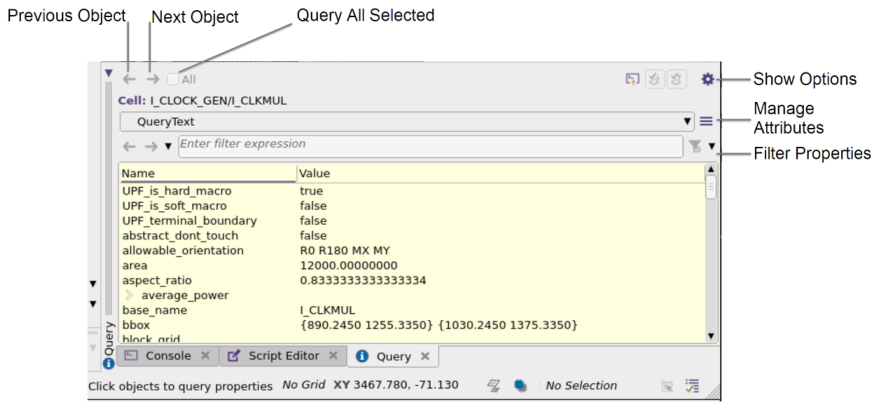
\includegraphics[width=0.92\textwidth]{gui-fig-022.png}
\caption{Query 面板}
\label{fig:gui-22}
\end{figure}

要显示某个对象的信息，单击该对象。工具会把该对象的信息填入 Query 面板。

要显示查询工具，并填入所选对象的信息，选择 \textbf{Select > Query Selection}。

要进一步控制 Query 面板中的信息显示，单击 Show Options 按钮并更改选项：
\begin{itemize}
  \item 选择 Auto Print Text to Log，则每次查询新对象时，把 Query 面板的内容写到控制台（console）。
  \item 选择 Auto Show when Query Tool is Chosen，则在 Query Tool 处于活动状态时，单击对象会自动打开 Query 面板。
  \item 单击 Customize Text，打开 Customize Query Toolbar 对话框。详见下文「使用定制查询工具栏」。
  \item 选择 Warn in selection exceeds size limit，并设置一个上限。选择规模超过该上限时，工具发出警告。
  \item 选择 Show attribute group，在 Query 面板中显示属性组（attribute group）选择框。
  \item 单击 Show attribute filter，在 Query 面板中显示文本过滤框。
\end{itemize}

在属性组框中选择一个属性组，则只显示属于该组的属性。要进一步了解某个组有哪些属性，单击属性组框右侧的 Activate Attribute Group Manager 按钮。属性组的说明见下文「使用属性组管理器」。

在过滤框中输入简单文本字符串，则只显示属性名中包含该文本的属性。要清除字符串，单击过滤文本框右侧的 (X)。单击过滤框右侧的 Filter properties 按钮，并选择 Show Read Only Properties，则只显示值为只读的属性。

单击 Name 或 Value 列标题，可更改该列的排序顺序。

\subsection{使用定制查询工具栏}
\subsubsection*{Using the Customize Query Toolbar}

要打开定制查询工具栏（Customize Query Toolbar），在 Query 面板的 Show Options 面板中单击 Customize Text。该工具栏见图~\ref{fig:gui-23}。

\begin{figure}[htbp]
\centering
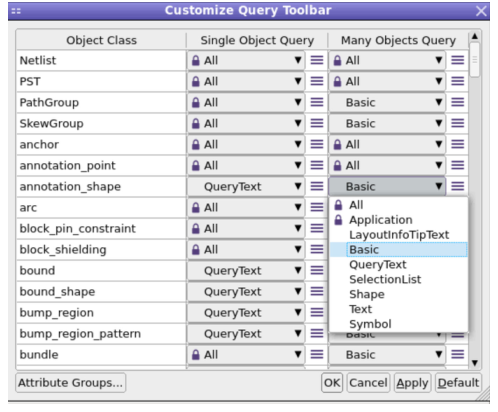
\includegraphics[width=0.55\textwidth]{gui-fig-023.png}
\caption{Customize Query Toolbar 对话框}
\label{fig:gui-23}
\end{figure}

Customize Query Toolbar 以表格显示对象类（Object Class）以及它们所属的属性组。要更改设置，单击 Single Object Query 或 Many Objects Query 列中的文本，并选择新值。选择 All，则该值会出现在所有组中。配置好列表后，单击 OK 或 Apply 使更改生效。

默认情况下，对象可以属于 Application、Basic、QueryText 等组。在 Query 面板中选中组名后，该对象类型的信息出现在 Query 面板的 Name 与 Value 列中。可以单击 Attribute Groups 按钮，用 Attribute Group Manager 对话框创建更多的组。详见下文「使用属性组管理器」。

\subsection{使用属性组管理器}
\subsubsection*{Using the Attribute Group Manager}

属性组管理器（Attribute Group Manager）用于定义新的属性组，以及向属性组添加对象或从中移除对象。

\begin{figure}[htbp]
\centering
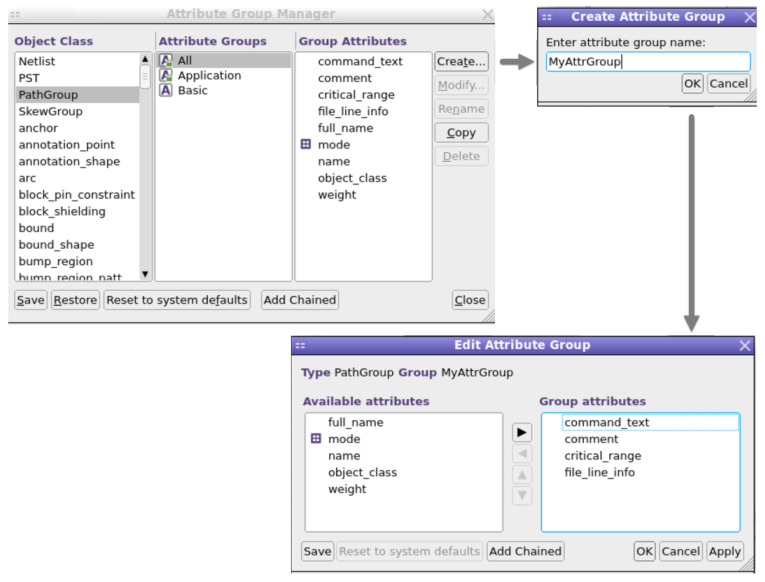
\includegraphics[width=0.85\textwidth]{gui-fig-024.png}
\caption{Attribute Group Manager 与 Attribute Group Editor}
\label{fig:gui-24}
\end{figure}

使用 Attribute Group Manager：
\begin{itemize}
  \item 单击 Create 创建新的属性组。在出现的对话框中输入属性组名称，单击 OK 保存。
  \item 单击某个 Object Class，再单击某个 Attribute Group 名称，然后单击 Modify，即可更改在 Query 面板中查询该对象时所显示的属性。详见下文「使用属性组编辑器」。
  \item 单击某个 Attribute Group 名称后再单击 Rename，或双击该 Attribute Group 名称，可重命名用户定义的属性组。系统定义的 Attribute Group 名称不能修改。
  \item 单击某个 Attribute Group 名称后再单击 Copy，可创建新的属性组，并把该组的属性复制到新属性组。
  \item 单击 Delete，从系统中移除所选的用户定义属性组。
  \item 单击 Save，把当前属性组设置写入 GUI 用户首选项文件。
  \item 单击 Restore，从 GUI 用户首选项文件读入属性组设置。
  \item 单击 Reset to system defaults，把应用程序定义的组内容恢复为默认值。用户定义的组不受影响。
\end{itemize}

\subsection{使用属性组编辑器}
\subsubsection*{Using the Attribute Group Editor}

属性组编辑器（Attribute Group Editor）用于向用户定义属性组的属性列表添加属性，或从中移除属性。在 Attribute Group Manager 中单击 Modify，即可打开 Attribute Group Editor。

按下列步骤修改所选属性组的属性列表：
\begin{itemize}
  \item 在左列选中一个属性，单击右箭头，把该条目移到右侧，使它可随此属性组一起显示。
  \item 在右列选中一个属性，单击左箭头，把该条目移到左侧，使它不在此属性组中使用。
  \item 在右列选中一个或多个条目，单击上箭头使条目在列表中上移；用下箭头使条目下移。
  \item 按 Control-A 选中该列中的全部条目。
  \item 单击 OK 保存结果，或单击 Cancel 退出对话框并且不保存。
\end{itemize}

\section{使用最近菜单按钮}
\subsection*{Using the Recent Menu Button}

最近菜单按钮（recent menu button）以图标和文字显示你在 GUI 中最近执行的操作。单击布局窗口左上方、当前鼠标工具图标下方的下箭头，即可显示该按钮，见图~\ref{fig:gui-25}。

\begin{figure}[htbp]
\centering
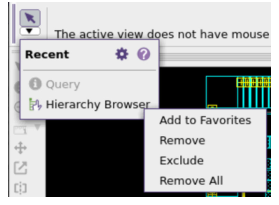
\includegraphics[width=0.4\textwidth]{gui-fig-025.png}
\caption{最近菜单按钮}
\label{fig:gui-25}
\end{figure}

在 GUI 中执行任务时，工具会在最近操作列表的顶部插入图标和文字。默认显示最近五条命令。单击 Show Options 按钮，为 Maximum Commands 选择新值，即可更改这个数目。

工具提供快捷键，用来调用最近使用的九条命令。按 Alt-1 调出最近一条命令，按 Alt-2 调出倒数第二条，其余依此类推。

可以右键单击，并从上下文菜单中选择下列选项，以修改最近使用命令的列表：
\begin{itemize}
  \item 选择 Add to Favorites，把该命令加入 Favorites 工具栏的命令列表。
  \item 单击 Remove，从最近使用命令列表中删除该命令。
  \item 单击 Exclude，删除该命令，并阻止它以后再进入此列表。要把命令从排除列表中移除，单击 Show Options 按钮，再单击 Reset Excluded。
  \item 单击 Remove All，从最近使用命令列表中移除全部命令。
\end{itemize}

单击 Show Options 按钮，可更改 Recent 工具栏的其他设置：
\begin{itemize}
  \item 用 Maximum Commands 为最近操作列表所保存的最大命令数选择新值。
  \item 单击 Reset Exclude，把全部命令从排除列表中移除。只有已经排除过一条或多条命令时，此按钮才可用。
\end{itemize}

\section{使用脚本编辑器}
\subsection*{Using the Script Editor}

脚本编辑器（Script Editor）用于在 IC Compiler II 中加载、编辑、运行和保存 Tcl 脚本。选择 \textbf{View > Toolbars > Script Editor} 即可激活。也可以把鼠标移到布局视图底部的状态栏，右键单击，从上下文菜单中选择 Script Editor。

\begin{figure}[htbp]
\centering
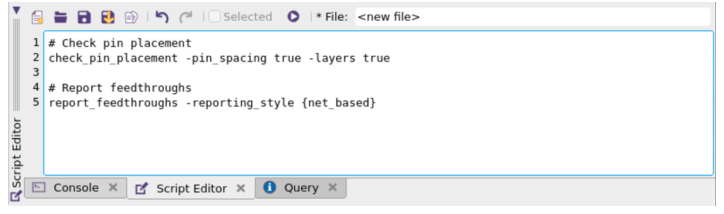
\includegraphics[width=0.85\textwidth]{gui-fig-026.png}
\caption{脚本编辑器}
\label{fig:gui-26}
\end{figure}

把指针移到图标上，信息提示（infotip）中会显示其功能。在 Script Editor 中可以做下列操作：
\begin{itemize}
  \item 单击 New，清除脚本窗口的内容。
  \item 单击 Open，在 Open 对话框中输入文件名，读入已有脚本。
  \item 单击 Save 保存脚本。
  \item 单击 Save As，用新文件名保存脚本。
  \item 单击 Undo，撤销对脚本的一处修改。
  \item 单击 Redo，反向最近一次撤销。
  \item 在搜索框中输入文本，单击 Find next 在文件中向前搜索；单击 Find previous 在脚本中向后搜索。
  \item 在搜索框中输入整数，单击 Go to line，把编辑器滚动到指定行号。
  \item 单击 Run Script，把脚本编辑器的内容保存到临时文件，并作为 Tcl 命令运行该文件。
  \item 用鼠标在脚本编辑器中选中单词或行，单击 Run Selection，把所选内容保存到文件并作为 Tcl 命令执行。
  \item 通过键入、剪切粘贴或删除文本，编辑脚本编辑器中的内容。
\end{itemize}

\section{使用按名称选择工具栏}
\subsection*{Using the Select By Name Toolbar}

按名称选择工具栏（Select By Name toolbar）按对象名称或搜索过滤表达式选择或高亮对象。选择 \textbf{Select > By Name Toolbar} 即可激活。也可以单击布局窗口左下角的 Select By Name 按钮。

\begin{figure}[htbp]
\centering
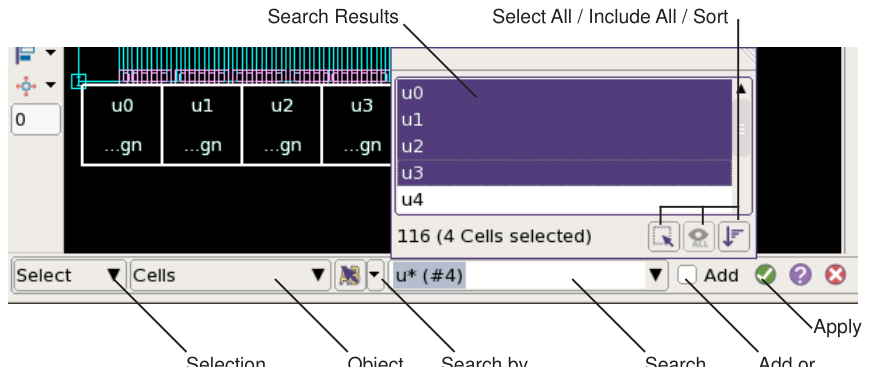
\includegraphics[width=0.92\textwidth]{gui-fig-027.png}
\caption{Select By Name 工具栏}
\label{fig:gui-27}
\end{figure}

该工具栏支持键盘快捷键，便于搜索并选择对象。使用 Select By Name 工具栏的典型流程如下：
\begin{enumerate}
  \item 按 Ctrl+/ 显示 Select By Name 工具栏。
  \item （可选）把选择模式改为 Highlight，以高亮（highlight）所选对象。
  \item （可选）从 Object Type 列表中选择对象类型。
  \item 按 F3 按名称搜索，或按 F4 按过滤器搜索。
  \item 输入与所找对象名称开头相匹配的部分搜索词。若没有匹配项，工具把输入框着成浅红色。
  \item 按 Tab，把搜索词扩展为匹配的对象名；若搜索词匹配多个对象，则显示全部匹配结果。
  \item 按 Insert，在 Add to Selection 与 Replace Selection 之间切换。
  \item 按 Enter 或单击 Apply，选中这些对象。
\end{enumerate}

\subsection{为多个对象输入搜索词}
\subsubsection*{Entering Search Terms for Multiple Objects}

搜索框提供灵活的界面，用来查找多个对象。要搜索多个对象名，用空格分隔搜索词。若对象名本身含有空格，用花括号 \cmd{\{\}} 分隔各项。按 Tab 键，搜索文本光标之前的那一项。要搜索另一项，移动光标后再按一次 Tab。单击搜索框右侧的 (X) 可清除搜索词。

若搜索词匹配多个对象，工具显示可滚动的搜索结果列表。继续键入，加长搜索词，以缩小结果范围。按上箭头键或下箭头键，在列表中向上或向下滚动。按 Enter 选中列表中的单个条目；按住 Control 键并单击其他结果，可把它们一并选中。单击 Select All 按钮，或按 Ctrl+A，选中列表中的全部结果。单击 Sort 按钮，反转列表的排序。按 Esc 退出列表。

在列表中选中多个对象后，搜索框显示缩写后的搜索词，例如 \cmd{(\#4)}，其中 4 是所选对象的个数。要在布局中选中这些对象，按 Enter。要把更多对象加入选择，单击 Add 选项或按 Insert，然后输入新的搜索词，并重复前面的步骤。

\subsection{按过滤器搜索}
\subsubsection*{Searching by Filter}

可以用 Select By Name 工具按过滤表达式搜索对象，见图~\ref{fig:gui-28}。

\begin{figure}[htbp]
\centering
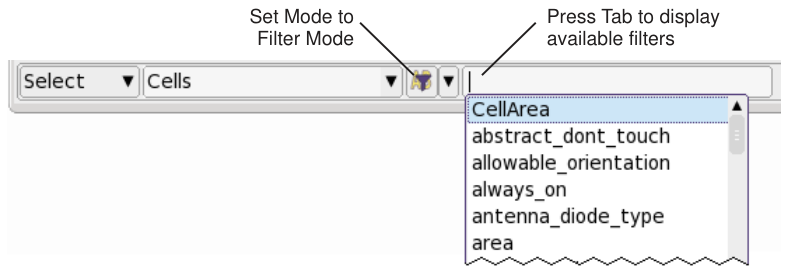
\includegraphics[width=0.85\textwidth]{gui-fig-028.png}
\caption{按过滤器选择}
\label{fig:gui-28}
\end{figure}

键入搜索表达式的前几个字母再按 Tab，即可快速构成过滤表达式。构成过滤搜索表达式的典型流程如下：
\begin{enumerate}
  \item 键入搜索表达式的前几个字母，例如 a。
  \item 按 Tab，显示与搜索表达式匹配的属性列表。
  \item 继续键入以缩小搜索范围，或单击列表中的属性。
  \item 再按 Tab，显示该属性的合法运算符。
  \item 继续键入以缩小搜索范围，或单击列表中的属性。
  \item 再按 Tab。若属性取枚举值（enumerated value），工具显示合法取值；否则在搜索框中插入一对空引号，或插入数值 0.0。
  \item 继续用 Tab 重复上述步骤，向表达式追加更多内容；或按 Enter 提交该表达式并执行搜索。
\end{enumerate}

\section{使用总览工具栏}
\subsection*{Using the Overview Toolbar}

总览工具栏（Overview toolbar）显示整个布局视图的轮廓，并用黄色高亮标出布局视图当前显示的区域。选择 \textbf{View > Toolbars > Overview}，即可激活总览工具栏并显示 Overview 面板。要在小弹出窗口中显示总览，单击布局窗口底部的 Overview 按钮。

\begin{figure}[htbp]
\centering
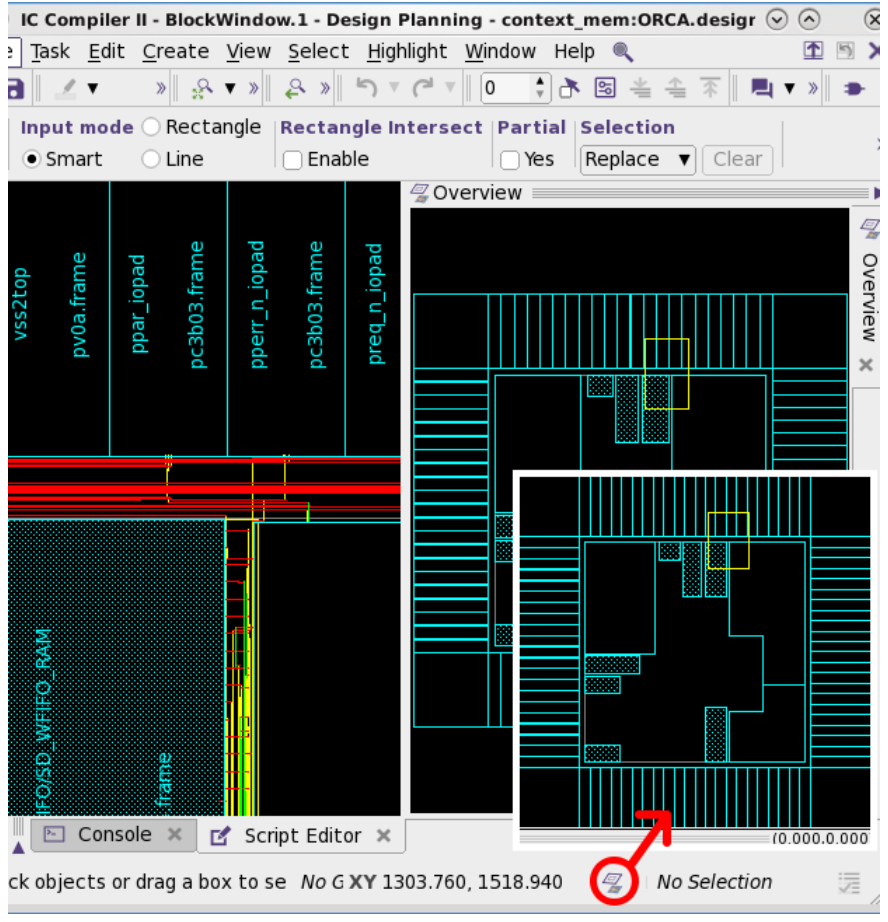
\includegraphics[width=0.92\textwidth]{gui-fig-029.png}
\caption{Overview 工具栏}
\label{fig:gui-29}
\end{figure}

要更改布局窗口中显示的设计区域，在总览面板或窗口中单击并拖拽黄色高亮区域。松开鼠标后，布局视图更新为高亮范围内的区域。

要更改布局视图的缩放倍数，把指针移到黄色高亮区域的边界。指针会变成可调整高亮大小的形状。单击并拖拽边缘，即可放大或缩小。

\section{使用选择列表与工作列表}
\subsection*{Using the Selection List and Work List}

选择列表（selection list）列出设计中当前选中的对象。若所选对象类型相同，选择列表显示这些对象的 Selection List 属性组。若对象类型不同，选择列表显示对象的 \cmd{name}、\cmd{object\_class} 与 \cmd{full\_name} 属性。

下图是选中了工作列表选项卡的 Selection List 对话框。

\begin{figure}[htbp]
\centering
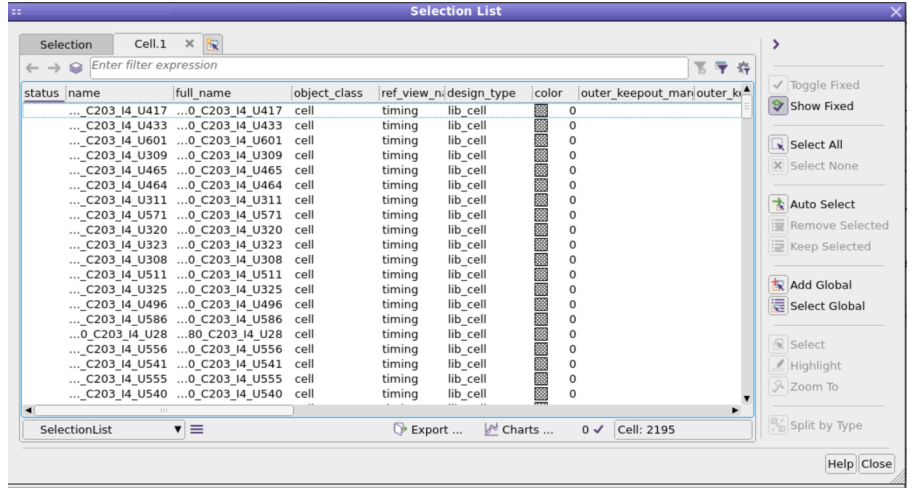
\includegraphics[width=0.92\textwidth]{gui-fig-030.png}
\caption{Selection List 对话框}
\label{fig:gui-30}
\end{figure}

选择列表中可以做下列操作：
\begin{itemize}
  \item 单击列标题，按该列对对象排序；再单击一次该标题，反转排序。
  \item 输入过滤表达式，减少列表中的条目。例如，下面的表达式只显示名称以 C 开头、朝向为 R270 的单元：
\end{itemize}

\begin{lstlisting}[language={}]
name=~C && orientation==R270
\end{lstlisting}

\begin{itemize}
  \item 单击过滤框旁的前后箭头，在以前用过的过滤表达式中向前或向后滚动。也可以单击过滤菜单按钮，查看全部过滤历史；单击列表中的一项，即用该表达式过滤列表。
  \item 单击 Toggle between filter expression 按钮，显示或隐藏各列自己的过滤器。
  \item 单击选项按钮，设置把过滤表达式解释为通配符表达式（wildcard expression）还是正则表达式（regular expression），以及多个表达式按 AND 组合还是按 OR 组合。
  \item 在属性组选择框中选择一项，为所选对象显示另一组列。默认显示 selection list 这一项。用 Attribute Group Manager 查看或修改某个属性组所显示的属性列表。
  \item 单击 Modify Attribute Group 按钮，以修改、管理或保存属性组。
  \item 单击 Charts 按钮，用图表分析设计数据。详见下文「图表」。
  \item 单击 Export 按钮，把列表或所选列表数据导出到 User Tables 导入表单，或导出为逗号分隔值（comma-separated values）文件。
\end{itemize}

\subsection{工作列表}
\subsubsection*{Work List}

工作列表（work list）是基于当前选择的持久对象列表。单击 Create Work List 选项卡按钮即可创建，此操作把当前选中的对象复制到工作列表。单击工作列表中的一项，会在当前布局、原理图或其他视图中自动选中该对象。工作列表的基本功能与选择列表相似，但在布局、原理图或其他视图中选择或取消选择对象时，工作列表保持不变。同一次工具会话中可以创建并管理多个工作列表，每个工作列表占用 Selection List 对话框中的一个选项卡。

工作列表选项卡中还可以做下列操作：
\begin{itemize}
  \item 选中一行或多行，单击 Toggle Selected Items Fixed 按钮，用勾号标记或取消标记这些项。
  \item 选中一行或多行，单击 Show/Hide Fixed Objects in List 按钮，显示或隐藏带勾号标注的行。
  \item 单击 Add Global Selection 按钮，把当前选中的项加入当前工作列表。
  \item 单击 Select Items to match Global Selection 按钮，在当前工作列表中选中那些同时在布局、原理图或其他视图中被选中的项。
\end{itemize}

\subsection{图表}
\subsubsection*{Charts}

要在图表中分析设计数据，单击 Selection List 对话框或工作列表选项卡中的 Charts 按钮，并从下列图表中选择：
\begin{itemize}
  \item Distribution plot：把一列的值划分到若干区间（bin）中，并显示每个区间内的值的个数。
  \item Box plot：按五数概括（five-number summary）显示一列或多列数值的分布。五数概括包括最小值（minimum）、第一四分位数（first quartile）、中位数（median）、第三四分位数（third quartile）与最大值（maximum）。位于 1.5 倍四分位范围（1.5 quartile range）之外的离群点（outlier）显示为单独的点。
  \item Scatter plot：在二维图中显示两列的值。
  \item Matrix plot：显示一组散点图。可以选择两列或多列，生成概括各列之间关系的图矩阵。
\end{itemize}

每个图表对话框都有上下文菜单，可对图执行常用操作。对话框中还包括：
\begin{itemize}
  \item 绘图区（plot area）
  \item 设置面板（settings panel）
  \item 数据表（data table，默认不显示）
  \item 状态栏（status bar）
\end{itemize}

可以指定图中使用的列、列分组（column group）、特定于该图的控件，以及选择行为的控件。

\section{使用用户表}
\subsection*{Using User Tables}

用户表（user table）用于导入、定义、交互操作并保存数据表。可以把用户表保存到设计数据库之外的文件中，并在以后的工具会话里重新加载。用户表可以由选择列表生成，也可以由逗号或制表符分隔的文件生成。

用户表支持许多常见的电子表格操作，例如编辑、排序、过滤、求和、查看列值分布等。此外，单击用户表中的行可以更改当前选择。

\subsection{创建用户表}
\subsubsection*{Creating a User Table}

从设计中已有的选择集创建用户表：
\begin{enumerate}
  \item 单击 Selection List 按钮，或选择 \textbf{Select > Selection List}，打开 Selection List 对话框。
  \item 单击 \textbf{Export > User Table}，按选择列表中的当前值创建用户表。\\
        工具把这些值复制到用户表导入表单。
  \item （可选）在 Table Name 框中更改表名。
  \item 单击 OK 导入数据并建立用户表。
\end{enumerate}

通过导入逗号或制表符分隔的文本文件创建用户表：
\begin{enumerate}
  \item 选择 \textbf{View > User Tables}。
  \item 单击用户表表单顶部附近的 Open 按钮。
  \item 在表单中选择分隔符（逗号或制表符）。需要时可以输入表名。
  \item 输入或选择文件名。
  \item 在 Configure Table Columns 表单中，按需要设置每一列的数据类型。
  \item 单击 OK 创建用户表。
\end{enumerate}

\subsection{保存与重新加载用户表}
\subsubsection*{Saving and Reloading a User Table}

保存用户表：
\begin{enumerate}
  \item 在表单顶部附近的 Action 框中选择 Save。
  \item 输入用于保存该数据库的文件名。用户表通常使用 \cmd{.utable} 扩展名。
  \item 单击 OK。
\end{enumerate}

工具把用户表数据写到指定文件。

加载已保存的用户表：
\begin{enumerate}
  \item 单击用户表表单顶部附近的 Open 按钮。
  \item 在 Select 下拉框中选择 Open UserTable file。
  \item 输入要加载的用户表文件名。
  \item 单击 OK。
\end{enumerate}

\subsection{分析用户表中的数据}
\subsubsection*{Analyzing Data in a User Table}

创建用户表之后，可以做下列操作：
\begin{itemize}
  \item 右键单击列标题，并选择上箭头或下箭头按钮，对该表排序或反向排序。
  \item 用下列方法之一过滤表：
  \begin{itemize}
    \item 单击过滤按钮；
    \item 在过滤栏中输入列迭代函数（iterator）与归约函数（reduction）。
  \end{itemize}
\end{itemize}

支持的函数包括：\cmd{approx()}、\cmd{abs()}、\cmd{round()}、\cmd{scale()}、\cmd{offset()}、\cmd{min()}、\cmd{max()}、\cmd{sum()}、\cmd{count()}、\cmd{avg()}、\cmd{mean()}、\cmd{median()}、\cmd{lower\_quartile()}、\cmd{uppper\_quartile()}、\cmd{stdev()}、\cmd{second\_stdev()} 与 \cmd{third\_stdev()}。

迭代函数的例子如下。它显示该表达式为真的所有行。用 \cmd{@column\_name} 语法引用列。

\begin{lstlisting}[language={}]
Tot Power > @Lkg Power
\end{lstlisting}

归约函数的例子如下。

\begin{lstlisting}[language={}]
Lkg\ Power > #mean(Tot\ Power)
\end{lstlisting}

下面的例子中，过滤查询显示某一行的 Tot Power 约等于同一行 Lkg Power 的 10\% 的所有行。

\begin{noteBox}
\cmd{approx()} 只能出现在表达式的右侧。
\end{noteBox}

还可以：
\begin{itemize}
  \item 单击并拖拽列标题，重排列的顺序。也可以右键单击列标题，选择 \textbf{More Column Options > Configure Columns}，打开 Configure Columns 对话框。
  \item 单击用户表表单顶部附近的 Tables 框并选择新的表名，以显示另一张用户表。
  \item 右键单击表中的单元格，选择 \textbf{Selection > Toggle Auto Select Mode}，再单击单元格，即可在布局或原理图视图中选择或取消选择当前对象。
\end{itemize}

\subsection{创建汇总报告}
\subsubsection*{Creating a Report Summary}

用户表中的汇总报告提供表列数据的基本统计。要为用户表生成汇总报告，在用户表表单顶部附近的 Action 框中选择 Report (summary)。工具显示表中数值列的统计量，包括最小值、最大值、平均值等。每一列的第一行给出该列数值与分类值的直方图（histogram）链接。

单击第一行中的任意链接，显示该列的分布报告。在分布报告中，单击列标题可按该列的值对表排序。在 Action 框中选择 Report (summary)，返回汇总报告。

\subsection{在用户表中自动选择对象}
\subsubsection*{Automatically Selecting Objects in a User Table}

可以用 Auto Select Object 下拉选项，让工具在用户表中自动选择对象。

默认选中 Objects defined by Column 与 None。其含义是：对于列中的某个值，工具按该列所定义的对象类型尝试选择对象。

若选择 Objects defined by object\_class，工具按对象类给出的对象类型，用 \cmd{full\_name} 列中的名称查找并选择对象。

\subsection{改进的总线压缩}
\subsubsection*{Improved Bus Compression}

可以压缩符合 \cmd{[*]} 总线记法、\cmd{[\#]}、\cmd{\_\#\_/} 或 \cmd{\_\#/} 的总线信号，其中 \# 为某个数字。

此选项可用于：
\begin{itemize}
  \item 任何含有线网、管脚、单元或时序点某种全名的列，作为列上下文菜单中的一项；
  \item hierarchy 视图与 Child List 视图。
\end{itemize}

该操作会创建一张用户表，把所有符合该总线记法的信号按总线合在一起。

单击 Show 列下方的某个链接，打开一张新的子表（child table），其中包含该总线上的各个信号。在这张子表中，若信号是时序路径的端点（endpoint），表中还可能有链接，用来查看时序路径点的子表。

用左上角的上下箭头，在下钻分析中生成的父表与子表之间来回切换。

\subsection{以图表或曲线查看数据}
\subsubsection*{Viewing the Data as a Chart or Plot}

要把用户表中的数据看成图表或曲线，使用列上下文菜单按钮 Select Plot。仅当所选列的数据包含数值时，该按钮才可用。

可以选中多列，再按用户表中这些列的数据创建图。

下图为生成的图。原稿未给出该图的 Figure 编号，图文件无法对应，故此处不插入图片。

要按列中的值过滤数据，把鼠标移到生成的图上并单击 Filter。可以用 Plot Control 定制并控制该图的各项选项。

要查看上次看过的图，单击 last viewed plot 工具按钮。只有此前查看过该表的图时，此按钮才可用。
